\documentclass[../ai_in_finance]{subfiles}
\usepackage[margin=1in]{geometry}
\usepackage{tikz}
\usetikzlibrary{positioning}
\usepackage{amsmath}
\usepackage{amssymb}
\usepackage{booktabs}
\usepackage{array}
\newcolumntype{L}[1]{>{\raggedright\arraybackslash}p{#1}}
\usepackage{url}
\usepackage{draftwatermark}

\SetWatermarkText{WSuo@Queensu.ca}
\SetWatermarkScale{1.4}
\SetWatermarkColor{gray!35}
\SetWatermarkAngle{45}

\usepackage{makeidx}
\makeindex

\begin{document}

\appendix
\chapter{Datasets and APIs for Financial AI}
\label{app:datasets}

\section{Introduction}

Every chapter in this book is built around a worked numerical example, and several of the later chapters, most notably Chapter 19's UCI credit-card default case study, are built around a real, publicly available dataset rather than a fictional one. This appendix collects, in one place, the data sources a reader is most likely to reach for when reproducing this book's examples with real data or extending them into an independent project: what each source covers, how it is typically licensed or priced, and the specific API or library used to pull it into Python.

This appendix is deliberately organized around \emph{access mechanism} as much as content, since the practical difference between a dataset a reader can query in five minutes with a free API key and one that requires an institutional subscription is often the difference between a project that gets started and one that does not. Where this book's own companion notebooks already reach outside the book's fictional running examples for real data, chiefly Chapter 5's CBOE Volatility Index (VIX) history (Section~\ref{sec:appendix-market-data}, downloaded live via the \texttt{yfinance} library) and Chapter 19's UCI ``Default of Credit Card Clients'' dataset (Section~\ref{sec:appendix-credit-data}), this appendix cross-references the relevant chapter directly.

\begin{figure}[htbp]
    \centering
    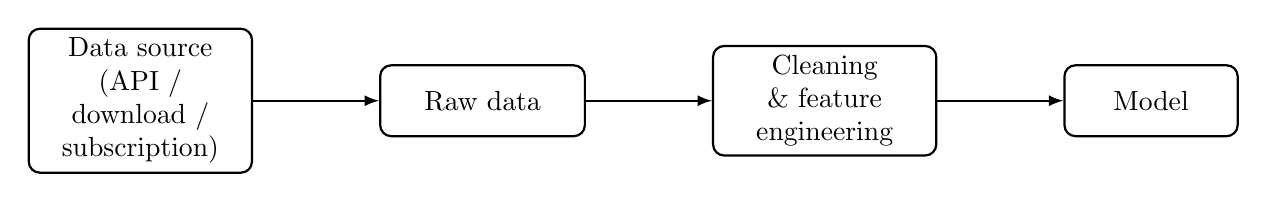
\begin{tikzpicture}[>=latex,thick,node distance=1.6cm]
        \node[draw,rounded corners,align=center,text width=2.6cm,minimum height=0.9cm] (source) {Data source (API / download / subscription)};
        \node[draw,rounded corners,align=center,minimum width=2.6cm,minimum height=0.9cm,right=of source] (raw) {Raw data};
        \node[draw,rounded corners,align=center,text width=2.6cm,minimum height=0.9cm,right=of raw] (clean) {Cleaning \& feature engineering};
        \node[draw,rounded corners,minimum width=2.2cm,minimum height=0.9cm,right=of clean] (model) {Model};
        \draw[->] (source) -- (raw);
        \draw[->] (raw) -- (clean);
        \draw[->] (clean) -- (model);
    \end{tikzpicture}
    \caption{Where the datasets and APIs in this appendix sit in a typical workflow: they supply the raw data, but the cleaning and feature-engineering steps introduced in Chapter 2's data-cleaning section and used throughout this book still have to be applied before the data reaches a model.}
    \label{fig:appendix-pipeline}
\end{figure}

\section{Market Price and Trading Data}
\label{sec:appendix-market-data}

\index{yfinance}Table~\ref{tab:appendix-market-data} summarizes the most commonly used sources for equity, index, foreign exchange, and derivatives price data. Yahoo Finance, accessed through the \texttt{yfinance} Python library, is the source this book itself uses: Chapter 5's implied-volatility section downloads the actual daily history of the VIX this way, with no API key required. It is an unofficial wrapper around Yahoo Finance's public website rather than a documented, versioned API, which is precisely why it is free; the tradeoff, discussed further in Section~\ref{sec:appendix-challenges}, is that it can change behavior or break without notice whenever Yahoo changes its own site.

\index{Refinitiv Datastream}Where CRSP and Compustat are US-centric, Refinitiv Datastream (a product of the London Stock Exchange Group since its 2021 acquisition of Refinitiv) is the closest institutional equivalent for international and cross-country work: decades of equity, index, bond, and FX price history across essentially every major market, not just the US, together with the Worldscope database of global company fundamentals bundled into the same platform. Like WRDS, it is licensed rather than freely available, typically through a university or employer subscription, and is accessed either through its legacy Excel add-in or through the Datastream Web Service (DSWS), a REST API with an official \texttt{DatastreamPy} Python client.

\begin{table}[htbp]
\centering
\caption{Market price and trading data sources.}
\label{tab:appendix-market-data}
\begin{tabular}{L{2.6cm}L{2.2cm}L{3.6cm}L{4.4cm}}
\toprule
Source & Access & API / library & Notes \\
\midrule
Yahoo Finance & Free & \texttt{yfinance} (PyPI) & Equities, ETFs, indices, FX, crypto, options chains; used in Chapter 5 of this book (the VIX example), and a natural real-data upgrade for Chapter 2's synthetic AssetA/AssetB series; unofficial, can break without notice \\
Alpha Vantage & Free tier + paid & REST API, key required (\url{alphavantage.co}) & Equities, FX, crypto, and technical indicators; free tier is rate-limited to a handful of calls per minute \\
Nasdaq Data Link (formerly Quandl) & Free + paid tiers & REST API (\url{nasdaqdatalink.com}) & Broad marketplace of market, commodity, and economic datasets from many contributors \\
Polygon.io & Free limited tier + paid & REST and WebSocket API & Real-time and historical US equities, options, FX, and crypto, including tick-level data \\
Tiingo & Free tier + paid & REST and WebSocket API & End-of-day prices, fundamentals, and news \\
CBOE DataShop & Paid & Web portal, bulk download & Official source for VIX methodology data and listed options data \\
WRDS: CRSP, TAQ & Institutional subscription (typically via a university) & Web query tool, plus SAS/Python/R client & CRSP is the academic gold standard for US equity returns; TAQ provides tick-by-tick trade and quote data used in Chapter 12's microstructure examples \\
Refinitiv Datastream (LSEG) & Institutional subscription (typically via a university or employer) & Excel add-in, or the Datastream Web Service (DSWS) REST API via \texttt{DatastreamPy} & The standard source for international/cross-country equity, index, bond, and FX history, plus Worldscope global fundamentals in the same platform; fills the gap CRSP and Compustat leave outside the US \\
\bottomrule
\end{tabular}
\end{table}

\section{Options and Derivatives Data}
\label{sec:appendix-options-data}

\index{OptionMetrics}Options data deserves its own treatment because it is structurally different from equity price data: a single underlying can have hundreds of simultaneously listed contracts across many strikes and expirations, and the quantity most useful for the work in Chapter 5 (pricing, the Greeks, implied volatility) and Chapter 8 (delta-normal and delta-gamma VaR for an options position) is not the raw quoted price but the implied volatility and Greeks computed from it, which not every source provides pre-computed.

OptionMetrics, accessed through WRDS as the IvyDB US database, is the main dataset academic options research is built on, occupying essentially the same role for options that CRSP occupies for equities (Section~\ref{sec:appendix-market-data}): daily, exchange-sourced, precomputed implied volatilities and Greeks for every listed US equity and index option going back to 1996, standardized enough that a result computed on it is directly comparable across studies. It is not free, licensed only through an institutional WRDS subscription, which is precisely why Table~\ref{tab:appendix-options} also lists several lighter-weight alternatives, from a free but shallow current-chain snapshot to paid practitioner-oriented vendors, for a reader without WRDS access.

\begin{table}[htbp]
\centering
\caption{Options and derivatives data sources.}
\label{tab:appendix-options}
\begin{tabular}{L{3.0cm}L{2.4cm}L{3.6cm}L{4.0cm}}
\toprule
Source & Access & API / library & Notes \\
\midrule
Yahoo Finance & Free & \texttt{yfinance}'s \url{Ticker.option_chain()} & Current listed option chains (bid, ask, volume, open interest) for a given expiration; no deep history, and implied volatility is Yahoo's own estimate rather than a modeled surface \\
CBOE DataShop & Paid & Web portal, bulk download & Official historical end-of-day and intraday options quotes directly from the exchange that lists most US index and equity options \\
Polygon.io Options API & Free limited tier + paid & REST and WebSocket API & Historical and real-time options chains with server-computed Greeks and implied volatility \\
WRDS: OptionMetrics (IvyDB US) & Institutional subscription & Web query tool, plus SAS/Python/R client & The academic standard for US options research: daily implied volatility surfaces and Greeks, precomputed, going back to 1996; directly usable for Chapters 5 and 8 \\
ORATS & Paid & REST API & Historical implied volatility surfaces, Greeks, and options analytics aimed at practitioners rather than academics \\
Deribit & Free, public endpoints & REST and WebSocket API, no key required for public data & The largest crypto options venue; full order book and historical settlement data for BTC and ETH options, useful for practicing the same Black-Scholes-Merton and Greeks machinery from Chapter 5 on an asset class with far higher realized volatility \\
CME DataMine & Paid & Bulk download / API & Historical futures and futures-options data (rates, commodities, equity index futures) directly from the exchange \\
\bottomrule
\end{tabular}
\end{table}

\section{Fundamental and Financial Statement Data}

\index{SEC EDGAR}The U.S. Securities and Exchange Commission's EDGAR system\index{Securities and Exchange Commission (SEC)} is the single most important free source of fundamental data for U.S. public companies, and it is directly relevant to Chapter 4's treatment of the income statement, balance sheet, and cash flow statement. Beyond the human-readable filings, the SEC exposes two machine-readable APIs at \url{data.sec.gov}: a full-text search API for locating specific language across filings (directly usable for Chapter 14's 10-K risk-factor classification example), and an XBRL ``company facts'' API that returns every structured financial figure, revenue, COGS, CFO, and so on, that a company has ever reported, tagged and time-stamped, for a given ticker or CIK (Central Index Key). Because these figures come directly from a company's own regulatory filings, they require no scraping or vendor licensing, only a descriptive \texttt{User-Agent} header identifying the requester, which the SEC requires of all automated EDGAR access.

\begin{table}[htbp]
\centering
\caption{Fundamental and financial statement data sources.}
\label{tab:appendix-fundamentals}
\begin{tabular}{L{3.0cm}L{2.2cm}L{3.6cm}L{4.0cm}}
\toprule
Source & Access & API / library & Notes \\
\midrule
SEC EDGAR & Free & REST API (\url{data.sec.gov}); full-text search and XBRL company-facts endpoints & Every US public company's own filings; ties directly to Chapters 4 and 14 \\
Financial Modeling Prep & Free tier + paid & REST API & Pre-parsed income statements, balance sheets, cash flow statements, and ratios \\
WRDS: Compustat & Institutional subscription & Web query tool, plus SAS/Python/R client & Standardized, restated fundamentals used throughout academic finance research \\
Macrotrends, StockAnalysis.com & Free (web only) & No official API & Convenient for spot-checking a single company's numbers by hand; not suitable for programmatic bulk use \\
\bottomrule
\end{tabular}
\end{table}

\section{Macroeconomic and Interest Rate Data}

\index{FRED (Federal Reserve Economic Data)}FRED, the Federal Reserve Bank of St. Louis's Federal Reserve Economic Data service, is the standard free source for the interest-rate and macroeconomic series this book uses conceptually in Chapter 5's term-structure discussion and Chapter 8's stress-testing scenarios. A free API key registered at \url{fred.stlouisfed.org} grants access to its REST API, and the community-maintained \texttt{fredapi} Python package wraps it in a single function call that returns a time-indexed \texttt{pandas} series, matching the data structures this book's notebooks already use throughout.

\begin{table}[htbp]
\centering
\caption{Macroeconomic and interest rate data sources.}
\label{tab:appendix-macro}
\begin{tabular}{L{3.0cm}L{2.2cm}L{3.6cm}L{4.0cm}}
\toprule
Source & Access & API / library & Notes \\
\midrule
FRED & Free, key required & REST API (\url{fred.stlouisfed.org}); \texttt{fredapi} package & Treasury yields, GDP, inflation, unemployment; directly usable for Chapters 5 and 8 \\
World Bank Open Data & Free & REST API (\url{worldbank.org}) & Global macro and development indicators across countries \\
IMF Data & Free & REST API & Global macro and financial-stability indicators \\
U.S. Bureau of Labor Statistics & Free, key optional & REST API (\url{bls.gov}) & US employment and price-inflation series \\
\bottomrule
\end{tabular}
\end{table}

\section{Credit, Lending, and Consumer Finance Data}
\label{sec:appendix-credit-data}

\index{UCI Machine Learning Repository}This is the category with the deepest overlap with this book's own worked examples. The UCI ``Default of Credit Card Clients'' dataset is already Chapter 19's own running case study, downloaded programmatically by that chapter's notebook rather than committed to this repository. The other datasets in Table~\ref{tab:appendix-credit} are natural extensions for the capstone project ideas Chapter 19 closes with.

\begin{table}[htbp]
\centering
\caption{Credit, lending, and consumer finance data sources.}
\label{tab:appendix-credit}
\begin{tabular}{L{3.4cm}L{2.2cm}L{3.6cm}L{3.4cm}}
\toprule
Source & Access & API / library & Notes \\
\midrule
UCI Default of Credit Card Clients & Free & Direct download via \texttt{urllib} & Chapter 19's own dataset; Taiwanese credit-card default data \\
UCI German Credit Data & Free & Direct download & Small, classic credit-scoring dataset, conceptually close to Chapter 6 and 9's examples \\
Lending Club loan data & Free (via Kaggle mirror) & Kaggle API & Loan-level peer-to-peer lending data; a Chapter 19 capstone idea \\
HMDA (Home Mortgage Disclosure Act) data & Free & REST API via the Consumer Financial Protection Bureau's data browser (\url{consumerfinance.gov}) & Mortgage application-level data widely used for fair-lending analysis; directly usable for Chapter 16's fairness audits \\
\bottomrule
\end{tabular}
\end{table}

\section{Fraud, AML, and Regulatory Compliance Data}

\index{IEEE-CIS Fraud Detection dataset}Genuinely labeled fraud data is scarce, since financial institutions rarely release real transaction-level fraud labels, which is exactly why the two datasets in Table~\ref{tab:appendix-fraud} recur so often in both industry benchmarks and this book's own Chapter 13 and Chapter 19 capstone list.

\begin{table}[htbp]
\centering
\caption{Fraud, AML, and regulatory compliance data sources.}
\label{tab:appendix-fraud}
\begin{tabular}{L{3.4cm}L{2.2cm}L{3.6cm}L{3.4cm}}
\toprule
Source & Access & API / library & Notes \\
\midrule
IEEE-CIS Fraud Detection (Kaggle) & Free (Kaggle competition dataset) & Kaggle API & Real, anonymized e-commerce transaction fraud data; a Chapter 13/19 capstone idea \\
PaySim & Free & Kaggle API & Synthetic mobile-money transaction data modeled on a real provider's logs; well suited to practicing the structuring and layering detection introduced in Chapter 13 \\
OFAC Sanctions Lists & Free & Bulk data files and a REST search API via the US Treasury & Sanctioned-party screening lists used in AML compliance workflows \\
\bottomrule
\end{tabular}
\end{table}

\section{Text, News, and Sentiment Data}

\index{Loughran-McDonald dictionary}Chapter 14's treatment of sentiment scoring rests on the Loughran-McDonald Master Dictionary, a word list purpose-built for financial text (ordinary sentiment dictionaries misclassify routine financial vocabulary, such as ``liability'' or ``tax,'' as negative), freely downloadable from its maintainer's University of Notre Dame page. Table~\ref{tab:appendix-text} lists this and the other text sources most relevant to that chapter.

\begin{table}[htbp]
\centering
\caption{Text, news, and sentiment data sources.}
\label{tab:appendix-text}
\begin{tabular}{L{3.4cm}L{2.2cm}L{3.6cm}L{3.4cm}}
\toprule
Source & Access & API / library & Notes \\
\midrule
SEC EDGAR full-text search & Free & REST API (\url{data.sec.gov}) & Search across filing text; directly usable for Chapter 14's 10-K risk-factor classification example \\
Loughran-McDonald Master Dictionary & Free & Direct CSV/text download & The sentiment word list underlying Chapter 14's scoring examples \\
Financial PhraseBank & Free & Hugging Face \texttt{datasets} library, or direct download & Sentence-level, analyst-labeled financial news sentiment \\
GDELT Project & Free & REST API and BigQuery access & Global news event and tone database, updated continuously \\
Reddit API & Free, registered app required, rate-limited & \texttt{praw} (Python Reddit API Wrapper) & Social sentiment data, e.g., retail-investor forums \\
X (formerly Twitter) API & Paid tiers & REST and streaming API & Social sentiment; access has moved to paid tiers since 2023, unlike the largely free access assumed by older tutorials \\
\bottomrule
\end{tabular}
\end{table}

\section{Alternative Data}

\index{alternative data}Chapter 15's case vignette on satellite-derived retail and commodity signals (RS Metrics, UBS, and Orbital Insight's oil-storage monitoring) is representative of this entire category: the underlying vendor data is almost always enterprise-priced and licensed rather than available through a simple API key, since it is expensive to produce and its main customers are institutional investors, not students. Table~\ref{tab:appendix-altdata} separates the handful of alternative-data sources that are genuinely free or low-cost from the enterprise vendors that are not, so a reader does not spend time chasing a free tier that does not exist.

\begin{table}[htbp]
\centering
\caption{Alternative data sources.}
\label{tab:appendix-altdata}
\begin{tabular}{L{3.0cm}L{2.6cm}L{3.6cm}L{3.2cm}}
\toprule
Source & Access & API / library & Notes \\
\midrule
Google Trends & Free, unofficial & \texttt{pytrends} (unofficial wrapper) & Search-interest series, often used as an attention or sentiment proxy \\
Orbital Insight, RS Metrics & Enterprise, paid & Vendor portal/API & Satellite-derived alternative data referenced in Chapter 15's case vignette; not accessible without a commercial contract \\
Similarweb, Sensor Tower & Paid & Vendor API & Web-traffic and app-usage panel data \\
MSCI ESG, Sustainalytics, Refinitiv ESG & Paid & Vendor API & ESG scores and underlying metrics \\
\bottomrule
\end{tabular}
\end{table}

\section{High-Frequency and Market Microstructure Data}

\index{LOBSTER}Reconstructing an actual limit order book, the exercise Chapter 3 introduces by hand and Chapters 11 and 12 build trading strategies on top of, requires message-level data that most retail-facing APIs simply do not provide. LOBSTER, an academic data service built on top of NASDAQ's own historical ITCH data, is the most accessible source of genuine, reconstructed limit-order-book data: it offers a free academic tier (typically a handful of sample days for a limited set of tickers) alongside paid access to its full history.

\begin{table}[htbp]
\centering
\caption{High-frequency and market microstructure data sources.}
\label{tab:appendix-hft}
\begin{tabular}{L{3.0cm}L{2.6cm}L{3.6cm}L{3.2cm}}
\toprule
Source & Access & API / library & Notes \\
\midrule
LOBSTER & Free academic tier + paid & Web portal, bulk download (\url{lobsterdata.com}) & Reconstructed limit order book data for NASDAQ-listed stocks; directly usable for Chapters 3, 11, and 12 \\
Databento & Pay-as-you-go & REST API, historical and live feeds & Modern, lower-cost alternative to legacy tick-data vendors for US equities, futures, and options \\
WRDS: NYSE TAQ & Institutional subscription & Web query tool, plus SAS/Python/R client & Tick-by-tick trade and quote data; the traditional academic source for Chapter 12-style microstructure research \\
\bottomrule
\end{tabular}
\end{table}

\section{Factor, Index, and Portfolio Data}

\index{Ken French Data Library}No source is more central to Chapter 10's factor-model examples than the Ken French Data Library, maintained by Dartmouth's Tuck School of Business, which has published the Fama-French factor returns (market, size, value, and their later extensions) and a large set of industry-sorted portfolios as free, direct-download CSV and ZIP files for over two decades. It has no formal REST API, but its file layout and URLs have been stable for so long that the \texttt{pandas-datareader} package includes a dedicated reader for it.

\begin{table}[htbp]
\centering
\caption{Factor, index, and portfolio data sources.}
\label{tab:appendix-factor}
\begin{tabular}{L{3.0cm}L{2.6cm}L{3.6cm}L{3.2cm}}
\toprule
Source & Access & API / library & Notes \\
\midrule
Ken French Data Library & Free & Direct CSV/ZIP download; also wrapped by \texttt{pandas-datareader} & Fama-French factor returns and industry portfolios; directly usable for Chapter 10 \\
iShares, SPDR ETF holdings & Free & Daily CSV download from the issuer's own website & Actual ETF basket composition; usable for Chapter 12's ETF-basket arbitrage example \\
S\&P Dow Jones Indices & Free (delayed) + paid (full) & Vendor portal & Index membership, methodology documents, and historical levels \\
\bottomrule
\end{tabular}
\end{table}

\section{Putting It Together: A Chapter-by-Chapter Dataset Map}

Table~\ref{tab:appendix-chapter-map} condenses the sections above into a single reference: for each chapter of this book, which of the sources above is the most natural place to look for real data to extend that chapter's fictional examples. Chapter 19's own closing list of capstone project ideas already names several of these sources directly; this table extends that same mapping to every other chapter.

\begin{table}[htbp]
\centering
\caption{A chapter-by-chapter map from this book's topics to the datasets and APIs most relevant to them.}
\label{tab:appendix-chapter-map}
\begin{tabular}{L{4.4cm}L{7.6cm}}
\toprule
Chapter & Most relevant data sources \\
\midrule
1. Introduction & (conceptual; no dataset needed) \\
2. Python for Finance & Yahoo Finance / \texttt{yfinance}, for real practice alongside the chapter's synthetic AssetA/AssetB series \\
3. Financial Markets and Institutions & LOBSTER (limit order book reconstruction), Yahoo Finance \\
4. Financial Statements & SEC EDGAR (filings and XBRL company facts) \\
5. Valuation and Asset Pricing & FRED (yield curve), Yahoo Finance / \texttt{yfinance} (already used for the VIX in Section~\ref{sec:appendix-market-data}), OptionMetrics or Deribit for real options chains (Section~\ref{sec:appendix-options-data}) \\
6. Machine Learning Fundamentals & UCI German Credit Data, or any dataset above used generically for classification practice \\
7. Time Series Analysis and Forecasting & FRED (macro series), Yahoo Finance (price series) \\
8. Market Risk Management & Yahoo Finance and FRED, for a real-portfolio VaR backtest; OptionMetrics or Polygon.io for a real delta-normal/delta-gamma VaR options example (Section~\ref{sec:appendix-options-data}) \\
9. Credit Risk Modeling & UCI Default of Credit Card Clients, Lending Club loan data, HMDA data \\
10. Portfolio Theory and Asset Allocation & Ken French Data Library, Yahoo Finance \\
11. Algorithmic Trading and Market Microstructure & LOBSTER, Yahoo Finance intraday data (where available) \\
12. High-Frequency Trading & LOBSTER, Databento, WRDS NYSE TAQ \\
13. Fraud Detection, Compliance, and Financial Crime & IEEE-CIS Fraud Detection, PaySim, OFAC sanctions lists \\
14. Natural Language Processing in Finance & SEC EDGAR full-text search, Loughran-McDonald dictionary, Financial PhraseBank, GDELT, Reddit API \\
15. Alternative Data and Deep Learning in Finance & Google Trends, satellite/alt-data vendors (enterprise), Similarweb \\
16. Explainability, Fairness, and Regulation & HMDA data, UCI Default of Credit Card Clients (as in Chapter 19's own capstone fairness audit) \\
17. Reinforcement Learning in Finance & Simulated market environments by design; LOBSTER or Yahoo Finance intraday data for a real extension of the chapter's execution and market-making agents \\
18. Agent-Based Models in Finance & Simulated agent populations by design; LOBSTER order-book data for a real zero-intelligence-trader comparison, or BIS locational banking statistics for a real interbank exposure network \\
19. Case Studies and Capstone Projects & The full list above; see Chapter 19's own closing section for specific project pairings \\
\bottomrule
\end{tabular}
\end{table}

\section{Practical Challenges in Sourcing Financial Data}
\label{sec:appendix-challenges}

Pulling real data into a project is rarely as simple as calling an API and moving on; several recurring problems are worth flagging explicitly.

\textbf{Point-in-time and look-ahead bias.} Most free APIs return a security's or company's data as it is known \emph{today}, not as it was actually known on the date being studied. Fundamentals get restated after the fact, index membership changes, and a company's own name or ticker can change; naively joining ``current'' fundamentals to historical prices silently leaks future information into a backtest, exactly the look-ahead-bias problem Chapter 15 raises directly.

\textbf{Survivorship bias.} A free API that only lists currently-traded tickers implicitly excludes every company that has since been delisted, gone bankrupt, or been acquired, which biases any historical universe built from it toward survivors. CRSP's paid, point-in-time data is the academic standard specifically because it avoids this.

\textbf{Licensing and redistribution restrictions.} Most vendor terms of service prohibit redistributing raw data even for non-commercial or educational use, which is exactly why this book's own real-dataset chapters (Chapter 19, and this appendix's own Chapter 5 VIX example) download data programmatically at run time rather than committing it to the repository. The same discipline is worth following in any derivative project.

\textbf{API and vendor instability.} Unofficial APIs such as \texttt{yfinance} work by interacting with a public website rather than a documented, contractually stable interface, so they can change behavior or stop working without notice whenever the underlying site changes. Even official free tiers are periodically discontinued or replaced outright, as has happened repeatedly across the market-data-vendor landscape. Every specific vendor and endpoint named in this appendix should therefore be treated as illustrative rather than permanent: verify current availability and terms directly with the provider before building anything on top of one.

\textbf{Rate limits and cost tiers.} Free tiers are typically rate-limited (a fixed number of calls per minute or per day), which matters when a project needs to pull data for hundreds of tickers rather than one; budgeting for a paid tier, or batching and caching requests locally, is often unavoidable at scale.

\section{Further Reading}

\begin{itemize}
\item U.S. Securities and Exchange Commission, \emph{EDGAR Application Programming Interfaces}, \url{sec.gov}.
\item Federal Reserve Bank of St. Louis, \emph{FRED API Documentation}, \url{fred.stlouisfed.org}.
\item Kenneth R. French, \emph{Data Library}, Tuck School of Business, Dartmouth College, \url{mba.tuck.dartmouth.edu}.
\item LOBSTER, \emph{Limit Order Book Data Documentation}, \url{lobsterdata.com}.
\item Kaggle, \emph{Datasets and Public API Documentation}, \url{kaggle.com}.
\item UCI Machine Learning Repository, \url{archive.ics.uci.edu}.
\item Loughran, T. and McDonald, B., ``When Is a Liability Not a Liability? Textual Analysis, Dictionaries, and 10-Ks,'' \emph{Journal of Finance}, 2011 (the paper underlying the Loughran-McDonald Master Dictionary).
\end{itemize}

\end{document}
